\label {fs-experiments}

To prove the feasibility of the proposed framework we conducted a series of experiments. We show the efficiency and scalability of the distributed streaming dataflow using latency and throughput as performance metrics. We also demonstrate that the introduced machine learning model is able to provide high accuracy together with reasonable training time. As a dataset, we used an open corpus of news articles from Russian media resource lenta.ru~\cite{lentaru}. This dataset contains about 700 000 documents, which are labeled by one of 90 different topics. In the experiments, we generated a stream consisted of articles from the dataset sorted by the time of publishing.

\begin{figure}[htbp]
  \centering
  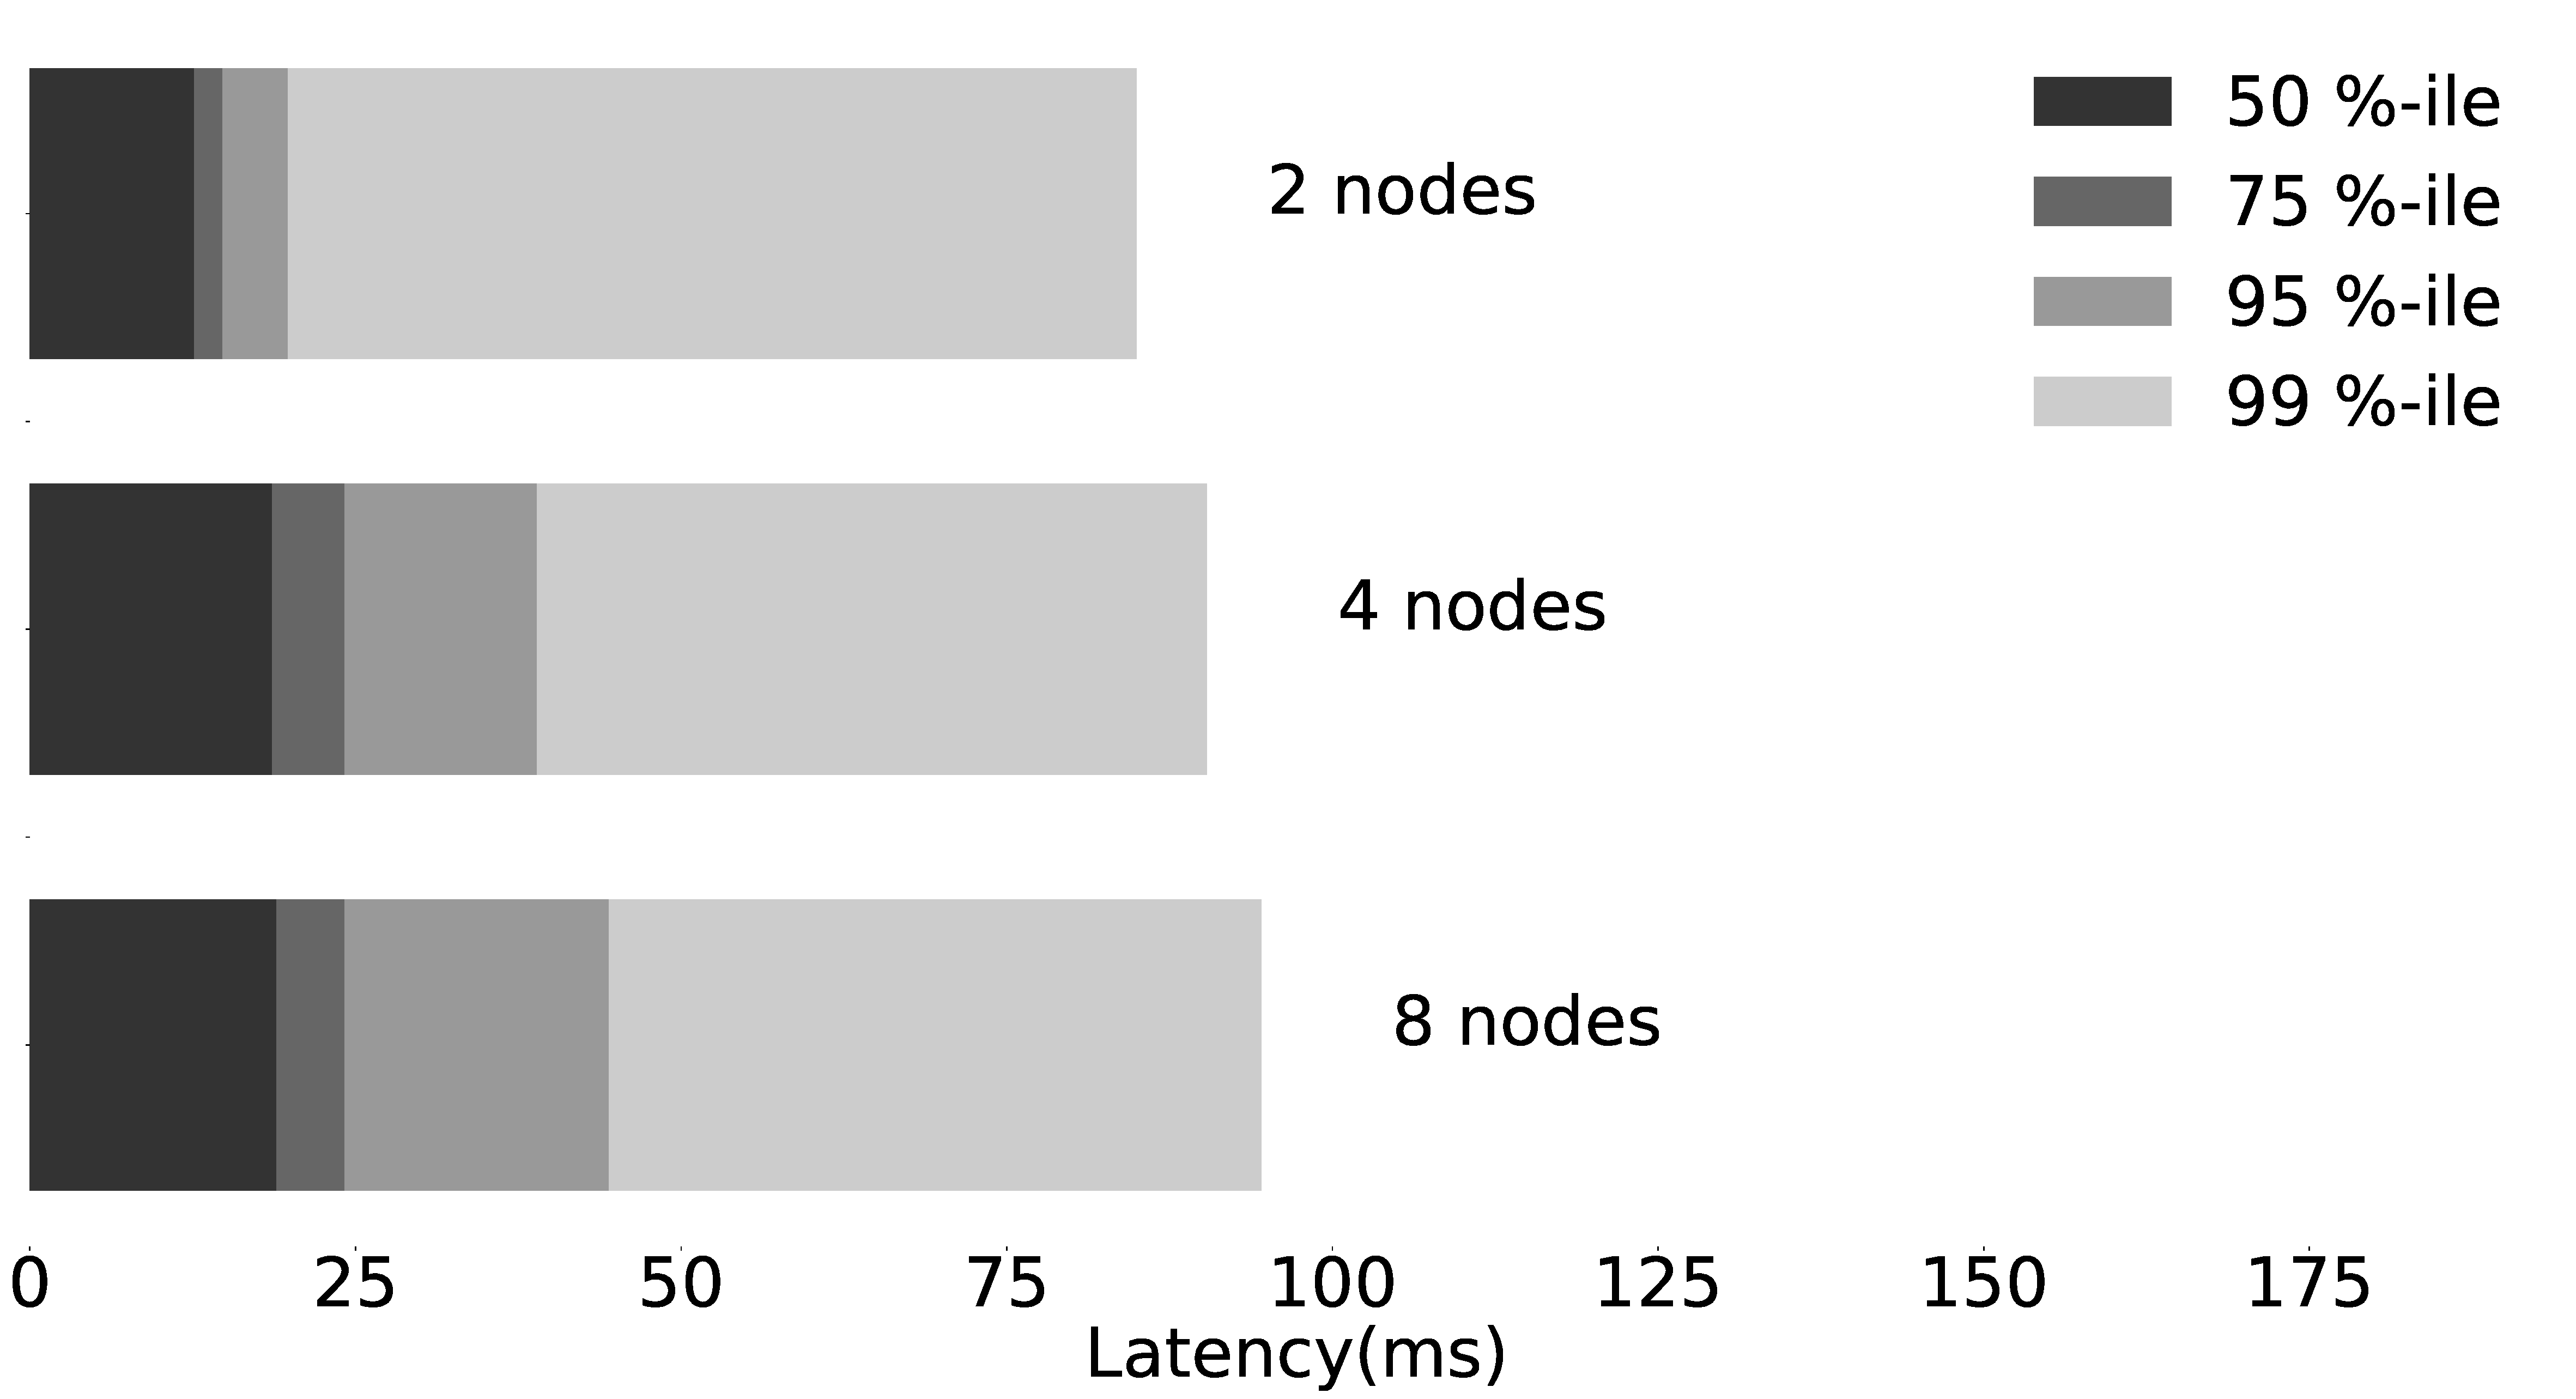
\includegraphics[scale=0.1]{pics/classifier_latencies}
  \caption{Classifier latencies}
  \label {latencies}
\end{figure}

\begin{figure}[htbp]
  \centering
  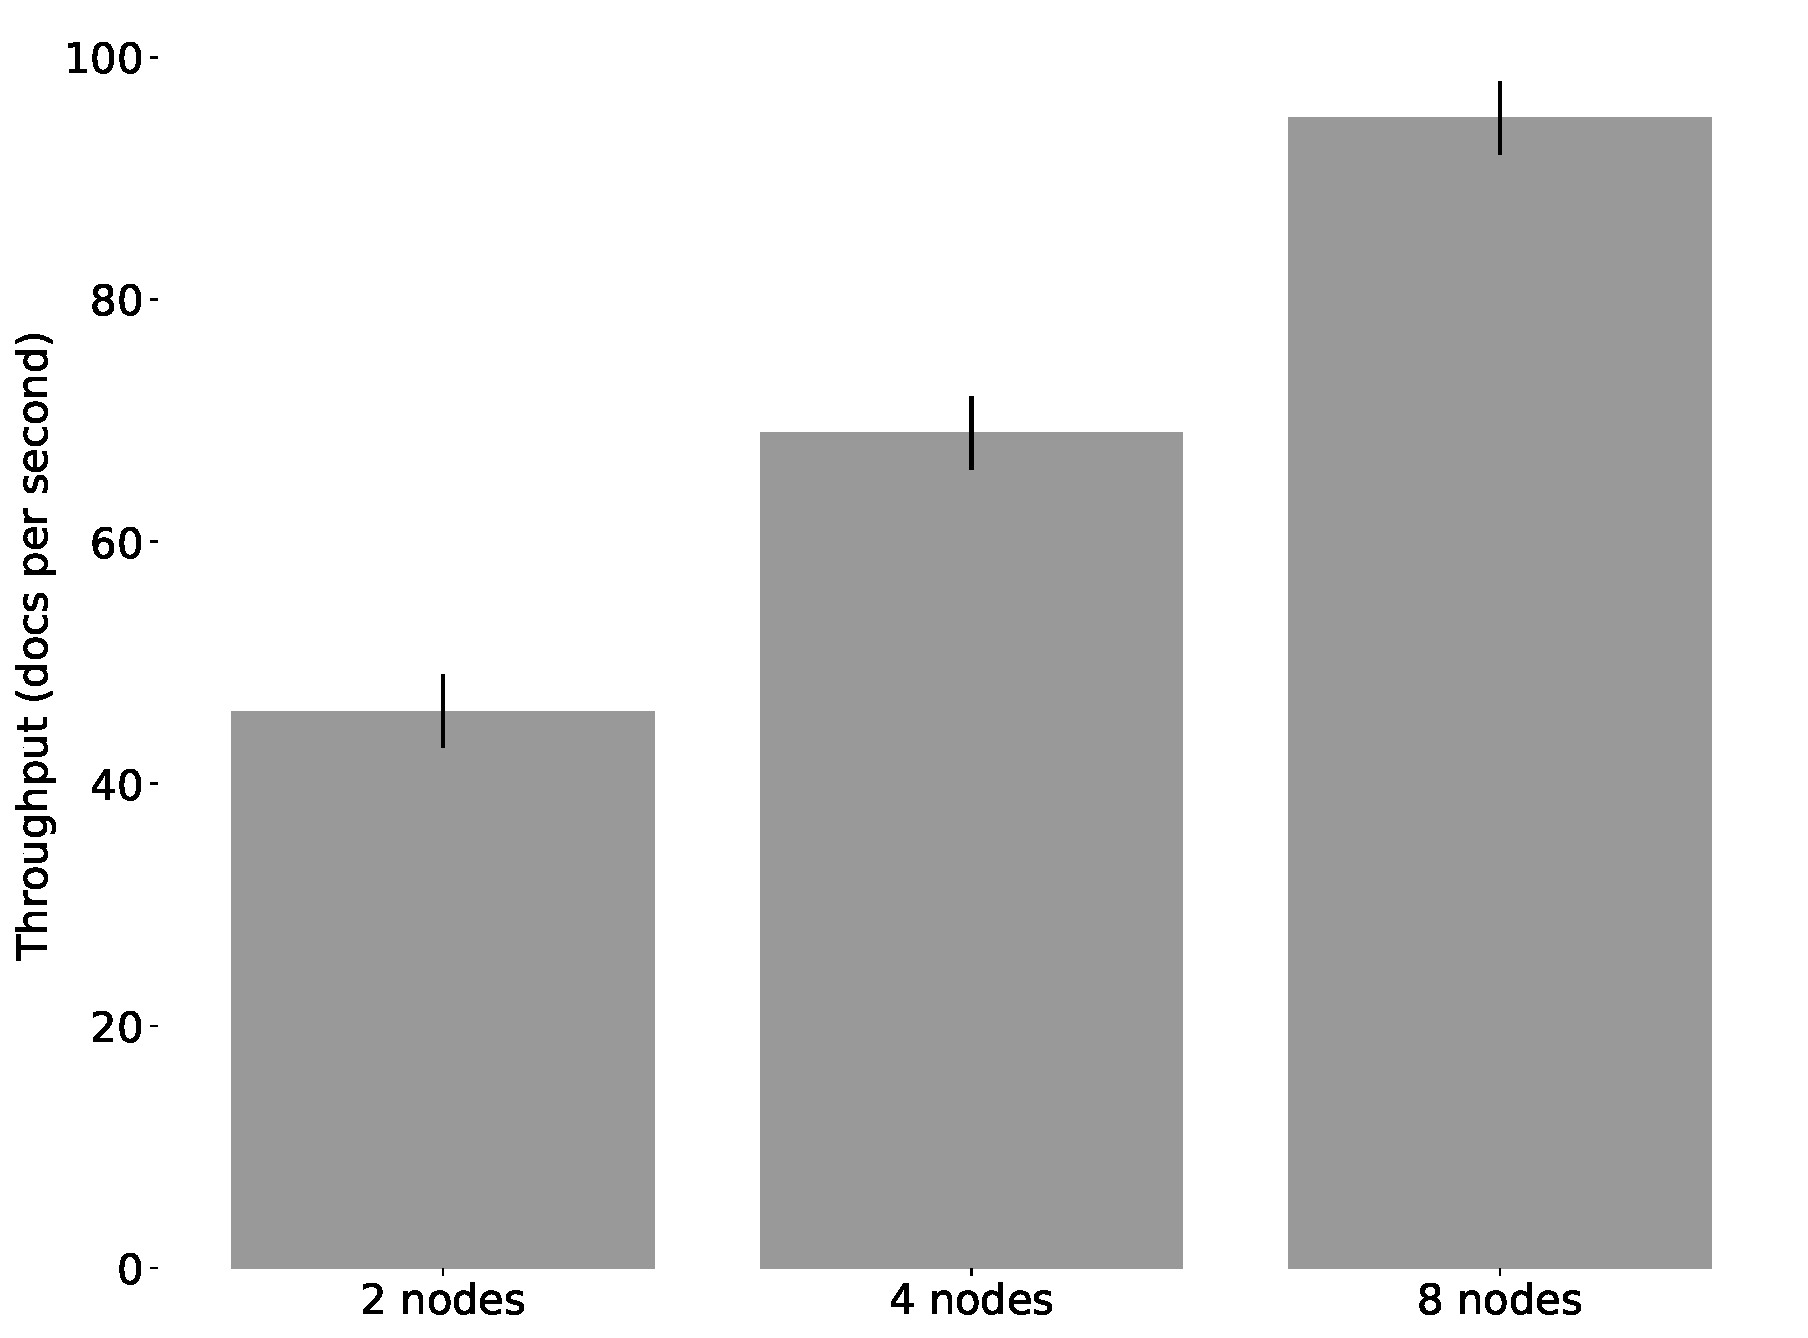
\includegraphics[scale=0.2]{pics/classifier_throughput}
  \caption{Classifier throughput}
  \label {throughput}
\end{figure}

\subsection{Data flow evaluation}

For evaluation, we deployed FlameStream on clusters, containing 2, 4 and 8 Amazon EC2 small instances with 2 GB of RAM and 1 core CPU. Exactly once guarantee was enabled and the period between state snapshots was 1 second. We measured throughput that is possible to achieve and the corresponding latency for prediction pipeline. The results are shown in Figures~\ref{latencies} and~\ref{throughput}. As we can see, there is a linear trend in throughput, which proves the scalability of the framework. On the other hand, one can observe, that latency increases moderately and keeps under 25 ms for a median and under 100 ms for 99th percentile. Insights on such an extremely low latency together with determinism and exactly once are given in~\cite{we2018beyondmr, we2018adbis}.

\subsection{Classifier evaluation}

To demonstrate the performance of the proposed machine learning model we compared two approaches. The first one is multinomial logistic regression with TF-IDF features computed on a complete dataset without $l2$ regularization. We denote it as a {\em static training}. The second one is dividing training dataset into relatively small batches and consequent applying MLR with $l2$ regularization to each batch with windowed TF-IDF features. The latter case demonstrates the behavior of our streaming classification approach. The results are shown in Table~\ref{accuracy}. The sizes of training and validations sets are 10 000 and 1000. As we can see, streaming approach outperforms static training. It indicates that our framework is able to handle the streaming nature of the news dataset including concept drift. The more formal rationale behind this fact is out of scope of this paper and relates to our future work.

\begin{table}[htbp]
\begin{tabular}{ll}
Method          & Accuracy \% \\
Static training  & 0.667          \\
Streaming training & 0.671         
\end{tabular}
\caption{Accuracy comparison between static and stream training}
\label{accuracy}
\end{table}